
\chapter{Appendix}
\section{Tabstopp-Logik}


Dieses Beispiel zeigt noch einmal, dass Coderedundanzen innerhalb
von mehreren Integrationen nichts Schlechtes sein muss.

Außerdem macht es auch deutlich, wie eine etwas komplexerer Integration mit
mehreren verschachtelten Lambda-Ausdrücken in der Praxis aussehen kann.

Mit Tab und Shift-Tab ist es dem Nutzer möglich den Tastaturfokus zu
verändern

Der nächsten Tabstopp soll nach folgenden Regeln und abhängig vom aktuell
fokussierten \textit{Model} bestimmt werden:

\begin{enumerate}
	\item FunctionUnit
	
	Besitzt aktuell die View einer FunctionUnit den Tastaturfokus, so soll als
	nächster Tabstopp der erste Datenfluss, der verbunden ist gewählt werden. Ist keiner
	verbunden, wähle als nächsten Tabstop den ersten Ausgang der Funktionseinheit.
	
	\begin{figure}[H]
		\centering
		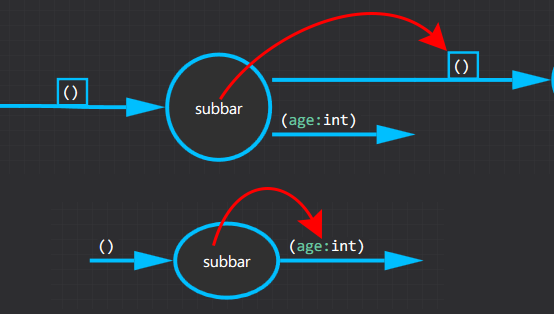
\includegraphics[width=0.6\linewidth]{./img/tabstop_functionunit.png}
		\caption{Aufgabe - Tabstopp von FunctionUnit aus}
	\end{figure}
	
	\item DataStream
	
	Wenn der Fokus aktuell auf einem DataStream liegt, so ist der nächste Tabstopp die Ziel-Funktionseinheit des Datenflusses.
	
	\begin{figure}[H]
		\centering
		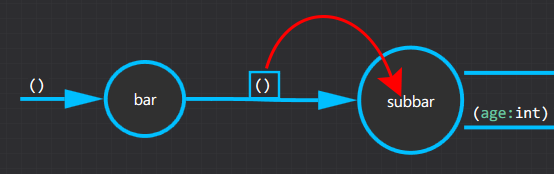
\includegraphics[width=0.6\linewidth]{./img/tabstop_datastream.png}
		\caption{Aufgabe - Tabstopp von DataStream aus}
	\end{figure}
	
	\item DataStreamDefinition
	
	Der komplexeste Fall: 
	Zu erst muss überprüft werden, ob es sich um ein Eingang oder Ausgang
	handelt. Ist es ein Eingang (A), so soll als nächster Tabstopp die Funktionseinheit
	zurückgegeben werden, von der die DataStreamDefinition der Eingang ist. 
	Bei einem Output muss überprüft werden, ob das Ende des Flows erreicht
	wurde, oder nicht. Wird ein verbundener Output entdeckt, wird der
	entsprechende DataStream als nächster Tabstopp zurückgegeben (B). Ist das Ende
	erreicht, so soll zum Anfang des kompletten Flows gesprungen werden (C).
	
	
	\begin{figure}[H]
		\centering
		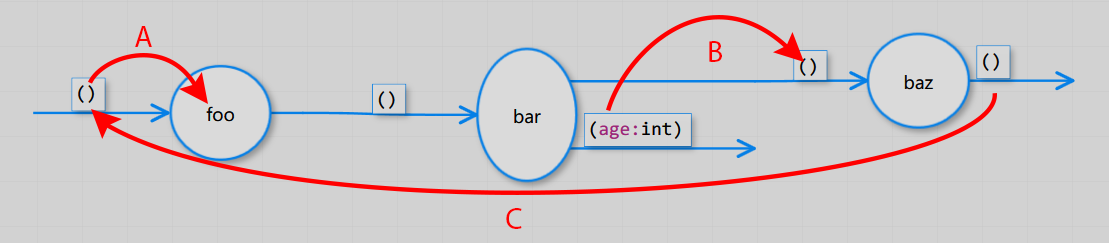
\includegraphics[width=\linewidth]{./img/tabstop_datastreamdefiniton.png}
		\caption{Aufgabe - Tabstopp von DataStreamDefinition aus}
	\end{figure}
	
	\begin{lstlisting}[caption=Tabstopp vorwärts]
	public static object TabStopGetNext(object focusedModel, MainModel mainModel)
	{
	object @return = null;
	
	focusedModel.TryCast<FunctionUnit>(fu =>
	{
	// prefer connected outputs as next tabstop
	// if no connected take first output defintion if there are any
	fu.OutputStreams.GetFirstConnected(
	foundConnected: connectedDsd => 
	@return =MainModelManager.FindDataStream(
	connectedDsd, mainModel),
	noConnected: () => 
	@return = fu.OutputStreams.FirstOrDefault());
	});
	
	focusedModel.TryCast<DataStream>(stream =>
	{
	// if focus was inside datastream take its destination function unit as next tabstop
	if (stream.Destinations.Any())
	@return = stream.Destinations.First().Parent;
	});
	
	focusedModel.TryCast<DataStreamDefinition>(dsd =>
	{
	// if focus was inside definition there are two case:
	// is input definition: next tabstop is the function unit of the definition
	// is output definition: in case the end of the flow was reached ( no connected output ) 
	// the next tabstop is the first input definition of the beginning of the whole flow.
	// Is the end not reached go to first connected output datastream
	dsd.CheckIsInputOrOutput( 
	isInput: () => @return = dsd.Parent,
	isOutput: () =>
	{
	dsd.Parent.OutputStreams.GetFirstConnected(
	foundConnected: connectedInput => 
	@return = MainModelManager.FindDataStream(
	connectedInput, mainModel),
	noConnected: () =>
	// loop tabstop focus when the 
	// end is reached
	@return = MainModelManager.GetBeginningOfFlow(
	dsd.Parent, mainModel)); 
	});
	});
	return @return;
	}
	
	\end{lstlisting}
	Analog dazu die Tabstopp-Methode in die entgegengesetzte Richtung.
	
	
	\begin{lstlisting}[caption=Tabstop rückwärts]
	public static object TabStopGetPrevious(object focusedModel, MainModel mainModel)
	{
	object @return = null;
	
	focusedModel.TryCast<FunctionUnit>(fu => 
	{
	fu.InputStreams.GetFirstConnected(
	foundConnected: connectedDsd => 
	@return = MainModelManager.FindDataStream(
	connectedDsd, mainModel),
	noConnected: () =>
	@return = fu.InputStreams.FirstOrDefault());
	});
	
	focusedModel.TryCast<DataStream>(stream => 
	{
	if (stream.Sources.Any())
	@return = stream.Sources.First().Parent;
	});
	
	focusedModel.TryCast<DataStreamDefinition>(dsd => 
	{
	dsd.CheckIsInputOrOutput(
	isOutput: () => @return = dsd.Parent,
	isInput: () => 
	{
	dsd.Parent.InputStreams.GetFirstConnected(
	foundConnected: connectedInput =>
	@return = MainModelManager.FindDataStream(
	connectedInput, mainModel),
	noConnected: () =>
	// loop tabstop focus when
	// the beginning is reached
	@return = MainModelManager.GetEndOfFlow(
	dsd.Parent, mainModel));
	});
	});	
	return @return;
	}
	\end{lstlisting}
	
	
	
	Auf oberster Ebene wird überprüft um welchen Typ von Objekt es sich
	handelt, der aktuell fokussiert ist \footnote{Teile davon war Aufgabe der UI und die
		Interaktion bekommt das Model dann als \texttt{object} übergeben. Deshalb bedarf es
		innerhalb der Methode einer Überprüfung des Typen mit TryCast. Natürlich
		könnte man dies auch durch ein Interface verhindern, dann würden die 3 Fälle
		jedoch nicht mehr klar vor einem liegen, sondern in den jeweiligen
		Implementierungen der Klassen versteckt.}. Nun existieren die drei Fälle, abhängig vom übergebenen Typen.\footnote{Zur Erinnerung: Die \texttt{Sources}-Eigenschaft eines \texttt{DataStream} beinhaltet nicht die Funktionseinheit,
		sondern die \texttt{DataStreamDefinition} einer Funktionseinheit. Die eigentliche
		Funktionseinheit enthält die \texttt{Parent}-Eigenschaft der \texttt{DataStreamDefinition}.
		Analog dazu enthält die \texttt{InputStream}- und \texttt{OutputStream}-Eigenschaft der
		Funktionseinheit auch nur die \texttt{DataStreamDefinition}-Objekte nicht ein \texttt{DataStream}-Objekt.
		Eine \texttt{DataStreamDefinition} kennt jedoch nicht den Datenfluss, mit dem sie
		verbunden ist. Eine Helfer-Methode der \texttt{MainModelManager}-Klasse stellt
		diese Funktionalität zum Auffinden des \texttt{DataStream} zur Verfügung.}
\end{enumerate}



